
\begin{figure}[ht]
  \centering
  \begin{tabular}{c c c c c }
    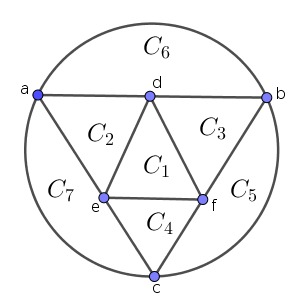
\includegraphics[width=3.5cm]{./img/octaCliques} &&   
    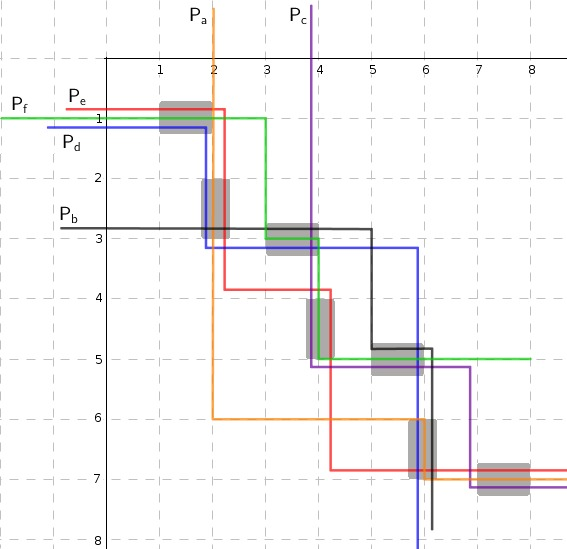
\includegraphics[width=9cm]{./img/representacaoLB}\\
    {\footnotesize (a) The octahedral graph $O_3$\vspace{.1cm}}&& 
    {\footnotesize (b) A Helly-EPG representation of the graph $O_3$} 
  \end{tabular}
  \caption{Helly-EPG representation of the graph $O_3$ according to the construction of Lemma~\ref{lem:todoGrafoEpgHelly}. The paths have been extended to the first/last row or column to improve the presentation.}\label{fig:gradeDemonstracao}
\end{figure} 
 